\documentclass[tikz,border=0cm]{standalone}
\usepackage{type1cm}
\usepackage{fp}
\usetikzlibrary{decorations.pathmorphing}
\usetikzlibrary{calc}
\usetikzlibrary{shadows}


\usepackage{fetamont}
\usepackage{cmbright}

\usepackage{bm,amsmath,amssymb}
\usepackage{soul}

\edef\myfontscale{1.2}
% \definecolor{simula}{RGB}{245,130,32}
% https://intranet.simula.no/sites/default/files/simula_rebrand_readme_2016.pdf
\definecolor{simula}{RGB}{241, 90, 34}
\definecolor{amaranth}{rgb}{0.9, 0.17, 0.31}
\definecolor{amber}{rgb}{1.0, 0.75, 0.0}

%% scalable vector fonts
\edef\fontSizeX{12}\edef\fontSizeY{14}
\FPupn{\resulttinyX}{myfontscale fontSizeX * 2 round}
\FPupn{\resulttinyY}{myfontscale fontSizeY * 2 round}
\renewcommand*{\tiny}{\fontsize{\resulttinyX}{\resulttinyY}\selectfont}

\edef\fontSizeX{14.4}\edef\fontSizeY{18}   
\FPupn{\resultscriptsizeX}{myfontscale fontSizeX * 2 round}
\FPupn{\resultscriptsizeY}{myfontscale fontSizeY * 2 round}
\renewcommand*{\scriptsize}{\fontsize{\resultscriptsizeX}{\resultscriptsizeY}\selectfont}

\edef\fontSizeX{17.28}\edef\fontSizeY{22}
\FPupn{\resultfootnotesizeX}{myfontscale fontSizeX * 2 round}
\FPupn{\resultfootnotesizeY}{myfontscale fontSizeY * 2 round}
\renewcommand*{\footnotesize}{\fontsize{\resultfootnotesizeX}{\resultfootnotesizeY}\selectfont}

\edef\fontSizeX{20.74}\edef\fontSizeY{25}
\FPupn{\resultsmallX}{myfontscale fontSizeX * 2 round}
\FPupn{\resultsmallY}{myfontscale fontSizeY * 2 round}
\renewcommand*{\small}{\fontsize{\resultsmallX}{\resultsmallY}\selectfont}

\edef\fontSizeX{24.88}\edef\fontSizeY{30}
\FPupn{\resultnormalsizeX}{myfontscale fontSizeX * 2 round}
\FPupn{\resultnormalsizeY}{myfontscale fontSizeY * 2 round}
\renewcommand*{\normalsize}{\fontsize{\resultnormalsizeX}{\resultnormalsizeY}\selectfont}

\edef\fontSizeX{29.86}\edef\fontSizeY{37}
\FPupn{\resultlargeX}{myfontscale fontSizeX * 2 round}
\FPupn{\resultlargeY}{myfontscale fontSizeY * 2 round}
\renewcommand*{\large}{\fontsize{\resultlargeX}{\resultlargeY}\selectfont}

\edef\fontSizeX{35.83}\edef\fontSizeY{45}
\FPupn{\resultLargeX}{myfontscale fontSizeX * 2 round}
\FPupn{\resultLargeY}{myfontscale fontSizeY * 2 round}
\renewcommand*{\Large}{\fontsize{\resultLargeX}{\resultLargeY}\selectfont}

\edef\fontSizeX{43}\edef\fontSizeY{54}
\FPupn{\resultLARGEX}{myfontscale fontSizeX * 2 round}
\FPupn{\resultLARGEY}{myfontscale fontSizeY * 2 round}
\renewcommand*{\LARGE}{\fontsize{\resultLARGEX}{\resultLARGEY}\selectfont}

\edef\fontSizeX{51.6}\edef\fontSizeY{64}
\FPupn{\resulthugeX}{myfontscale fontSizeX * 2 round}
\FPupn{\resulthugeY}{myfontscale fontSizeY * 2 round}
\renewcommand*{\huge}{\fontsize{\resulthugeX}{\resulthugeY}\selectfont}

\edef\fontSizeX{61.92}\edef\fontSizeY{77}
\FPupn{\resultHugeX}{myfontscale fontSizeX * 2 round}
\FPupn{\resultHugeY}{myfontscale fontSizeY * 2 round}
\renewcommand*{\Huge}{\fontsize{\resultHugeX}{\resultHugeY}\selectfont}

\edef\fontSizeX{74.3}\edef\fontSizeY{93}
\FPupn{\resultveryHugeX}{myfontscale fontSizeX * 2 round}
\FPupn{\resultveryHugeY}{myfontscale fontSizeY * 2 round}
\newcommand*{\veryHuge}{\fontsize{\resultveryHugeX}{\resultveryHugeY}\selectfont}

\edef\fontSizeX{89.16}\edef\fontSizeY{112}
\FPupn{\resultVeryHugeX}{myfontscale fontSizeX * 2 round}
\FPupn{\resultVeryHugeY}{myfontscale fontSizeY * 2 round}
\newcommand*{\VeryHuge}{\fontsize{\resultVeryHugeX}{\resultVeryHugeY}\selectfont}

\edef\fontSizeX{107}\edef\fontSizeY{134}
\FPupn{\resultVERYHugeX}{myfontscale fontSizeX * 2 round}
\FPupn{\resultVERYHugeY}{myfontscale fontSizeY * 2 round}
\newcommand*{\VERYHuge}{\fontsize{\resultVERYHugeX}{\resultVERYHugeY}\selectfont}

% set the normalfont (default)
\renewcommand*{\normalfont}{\normalsize}
% !TEX root = tesi.tex
\newcommand{\R}{\mathbb{R}}
\newcommand{\Cfield}{\mathbb{C}}
\newcommand{\vect}[1]{\mathbf{#1}}
\newcommand{\tens}[1]{\mathsf{#1}}
% something between bar and overline
%\newcommand{\overbar}[1]{\mkern 1.5mu\overline{\mkern-1.5mu#1\mkern-1.5mu}\mkern 1.5mu}
\makeatletter
\newsavebox\myboxA
\newsavebox\myboxB
\newlength\mylenA
\newcommand*\overbar[2][1.00]{%
    \sbox{\myboxA}{$\m@th#2$}%
    \setbox\myboxB\null% Phantom box
    \ht\myboxB=\ht\myboxA%
    \dp\myboxB=\dp\myboxA%
    \wd\myboxB=#1\wd\myboxA% Scale phantom
    \sbox\myboxB{$\m@th\overline{\copy\myboxB}$}%  Overlined phantom
    \setlength\mylenA{\the\wd\myboxA}%   calc width diff
    \addtolength\mylenA{-\the\wd\myboxB}%
    \ifdim\wd\myboxB<\wd\myboxA%
       \rlap{\hskip 0.5\mylenA\usebox\myboxB}{\usebox\myboxA}%
    \else
        \hskip -0.5\mylenA\rlap{\usebox\myboxA}{\hskip 0.5\mylenA\usebox\myboxB}%
    \fi}
\makeatother

\newcommand{\vx}{\vect{x}}
\newcommand{\vy}{\vect{y}}
\newcommand{\vX}{\vect{X}}
\newcommand{\vA}{\vect{A}}
\newcommand{\va}{\vect{a}}
\newcommand{\vvb}{\vect{b}}
\newcommand{\vc}{\vect{c}}
\newcommand{\vk}{\vect{k}}
\newcommand{\ve}{\vect{e}}
\newcommand{\vp}{\vect{p}}
\newcommand{\vu}{\vect{u}}
\newcommand{\vv}{\vect{v}}
\newcommand{\vb}{\vect{b}}
\newcommand{\vf}{\vect{f}}
\newcommand{\vs}{\vect{s}}
\newcommand{\vg}{\vect{g}}
\newcommand{\vn}{\vect{n}}
\newcommand{\vm}{\vect{m}}
\newcommand{\vh}{\vect{h}}
\newcommand{\vt}{\vect{t}}
\newcommand{\vw}{\vect{w}}
\newcommand{\vfo}{\vf_\circ}
\newcommand{\vso}{\vs_\circ}
\newcommand{\vno}{\vn_\circ}

\newcommand{\vxi}{\bm{\xi}}

\newcommand{\tF}{\tens{F}}
\newcommand{\tT}{\tens{T}}
\newcommand{\tP}{\tens{P}}
\newcommand{\tS}{\tens{S}}
\newcommand{\tI}{\tens{I}}
\newcommand{\tQ}{\tens{Q}}
\newcommand{\tB}{\tens{B}}
\newcommand{\tC}{\tens{C}}
\newcommand{\tE}{\tens{E}}
\newcommand{\tR}{\tens{R}}
\newcommand{\tU}{\tens{U}}
\newcommand{\tA}{\tens{A}}
\newcommand{\tD}{\tens{D}}
\newcommand{\tH}{\tens{H}}
\newcommand{\tJ}{\tens{J}}
\newcommand{\tX}{\tens{X}}
\newcommand{\tV}{\tens{V}}
\newcommand{\tM}{\tens{M}}
\newcommand{\tL}{\tens{L}}

\newcommand{\tFiso}{\tF_\mathsf{iso}}
\newcommand{\tFvol}{\tF_\mathsf{vol}}

\newcommand{\tTiso}{\tT_\mathsf{iso}}
\newcommand{\btTiso}{\overbar[0.75]{\tT}_\mathsf{iso}}
\newcommand{\tTvol}{\tT_\mathsf{vol}}

\newcommand{\tSiso}{\tS_\mathsf{iso}}
\newcommand{\btSiso}{\overbar[0.9]{\tS}_\mathsf{iso}}
\newcommand{\tSvol}{\tS_\mathsf{vol}}

\newcommand{\tCiso}{\tC_\mathsf{iso}}
\newcommand{\tEiso}{\tE_\mathsf{iso}}
\newcommand{\tBiso}{\tB_\mathsf{iso}}
\newcommand{\vfiso}{\vf_\mathsf{iso}}
\newcommand{\vsiso}{\vs_\mathsf{iso}}
\newcommand{\cIiso}{\cI^\mathsf{iso}}

\newcommand{\tFa}{\tF_\mathsf{a}}
\newcommand{\tFe}{\tF_\mathsf{e}}
\newcommand{\tauref}{\tau_{\textsf{ref}}}
\newcommand{\tPa}{\tP_\mathsf{a}}
\newcommand{\tPe}{\tP_\mathsf{e}}
\newcommand{\tTa}{\tT_\mathsf{a}}
\newcommand{\tTe}{\tT_\mathsf{e}}
\newcommand{\tSa}{\tS_\mathsf{a}}
\newcommand{\tSe}{\tS_\mathsf{e}}
\newcommand{\tBe}{\tB_\mathsf{e}}
\newcommand{\tCe}{\tC_\mathsf{e}}

\newcommand{\sSa}{s_\mathsf{a}}
\newcommand{\bsSa}{\overbar s_\mathsf{a}}

\newcommand{\htSa}{\widehat\tS_\textsf{a}}

\newcommand{\body}{\mathfrak{B}}

\newcommand{\vphi}{\bm{\varphi}}
\newcommand{\veta}{\bm{\eta}}
\newcommand{\vvphi}{\hm{\varphi}}
\newcommand{\vTheta}{\bm{\Theta}}
\newcommand{\vpp}{\mathbf{p}}

\newcommand{\tK}{\tens{K}}
\newcommand{\tO}{\tens{O}}
\newcommand{\tKuu}{\tK_\mathsf{\varphi\varphi}}
\newcommand{\tKup}{\tK_\mathsf{\varphi p}}
\newcommand{\tKpu}{\tK_\mathsf{p \varphi}}
\newcommand{\tKpt}{\tK_\mathsf{p \theta}}
\newcommand{\tKtp}{\tK_\mathsf{\theta p}}
\newcommand{\tKtt}{\tK_\mathsf{\theta\theta}}
\newcommand{\tKpp}{\tK_\mathsf{pp}}
\newcommand{\vrhs}{\bm{\mathsf{f}}}
\newcommand{\vrhsu}{\vrhs_\mathsf{\varphi}}
\newcommand{\vrhst}{\vrhs_\mathsf{\theta}}
\newcommand{\vrhsp}{\vrhs_\mathsf{p}}

\newcommand{\cW}{\mathcal{W}}
\newcommand{\hcW}{\widehat\cW}
\newcommand{\tcW}{\widetilde\cW}
\newcommand{\hcWorth}{\hcW_\mathsf{orth}}
\newcommand{\hcWtr}{\hcW_\mathsf{tr}}
\newcommand{\cWiso}{\cW_\mathsf{iso}}
\newcommand{\hcWiso}{\hcW_\mathsf{iso}}
\newcommand{\cWvol}{\cW_\mathsf{vol}}
\newcommand{\cG}{\mathscr{G}}
\newcommand{\cGorth}{\cG_\mathsf{orth}}
\newcommand{\cGtr}{\cG_\mathsf{tr}}

\newcommand{\cI}{\mathcal{I}}

\newcommand{\aaf}{a_\mathsf{f}}
\newcommand{\aas}{a_\mathsf{s}}
\newcommand{\bbf}{b_\mathsf{f}}
\newcommand{\bbs}{b_\mathsf{s}}
\newcommand{\aafs}{a_\mathsf{fs}}
\newcommand{\bbfs}{b_\mathsf{fs}}

\newcommand{\CC}{\mathbb{C}}
\newcommand{\CCiso}{\CC_\mathsf{iso}}
\newcommand{\cc}{\mathfrak{c}}
\newcommand{\cciso}{\cc_\mathsf{iso}}
\newcommand{\ccvol}{\cc_\mathsf{vol}}
\newcommand{\bcciso}{\overbar{\cc}_\mathsf{iso}}

\newcommand{\tsp}[1]{#1^\mathsf{T}}
\newcommand{\mtsp}[1]{#1^{-\mathsf{T}}}
\newcommand{\dd}{\mathrm{d}}
\newcommand{\DD}{\mathrm{D}}

\newcommand{\eps}{\varepsilon}

\newcommand{\bracket}[1]{\left\langle #1 \right\rangle}
\newcommand{\norm}[1]{\left\Vert #1 \right\Vert}

\newcommand{\Piext}{\Pi_\mathsf{ext}}

\newcommand{\Lin}{\mathrm{Lin}}
\newcommand{\Linp}{\mathrm{Lin}^+}
\newcommand{\Orth}{\mathrm{Orth}}
\newcommand{\Orthp}{\mathrm{Orth}^+}
\newcommand{\Symp}{\mathrm{Sym}^+}

\newcommand{\ddV}{\dd V}
\newcommand{\ddv}{\dd v}
\newcommand{\ddA}{\dd A}
\newcommand{\dda}{\dd a}

\newcommand{\Vinner}{V_\mathsf{inner}}
\newcommand{\pinner}{p_\mathsf{inner}}

%\DeclareMathOperator{\diver}{div}
%\DeclareMathOperator{\tr}{tr}
%\DeclareMathOperator{\cof}{cof}
%\DeclareMathOperator{\dev}{dev}
%\DeclareMathOperator{\vol}{vol}
%\DeclareMathOperator{\DIV}{\textsc{Div}}
%\DeclareMathOperator{\DEV}{\textsc{Dev}}
%\DeclareMathOperator{\GRAD}{\textsc{Grad}}
%\DeclareMathOperator{\sym}{sym}
%\DeclareMathOperator{\diag}{diag}
%\DeclareMathOperator{\sign}{sign}

%\DeclareMathOperator*{\esssup}{ess\kern3pt sup}

\newcommand{\fcubic}{f_\mathsf{cubic}}
\newcommand{\fstep}{f_\mathsf{step}}
%\DeclareMathOperator{\Heavi}{\mathcal{H}}

\newcommand{\Cm}{C_\textsf{m}}
\newcommand{\Iionic}{I_\textsf{ionic}}
\newcommand{\Isource}{I_\textsf{source}}



\usepackage{booktabs,dcolumn}
\usepackage{array}
\newcolumntype{T}{>{\begingroup\bfseries}r<{\endgroup}}
\newcolumntype{N}{D{.}{.}{-1}}
\newcolumntype{R}{D{.}{.}{2.4}}
\newcolumntype{K}{D{.}{.}{3.4}}
\newcommand{\imgcase}[2]{\includegraphics[width=0.5\linewidth]{#1_#2_base}%
\includegraphics[width=0.5\linewidth]{#1_#2_side}}
\usepackage[tableposition=top,font=footnotesize,labelfont=bf,sf]{caption}

\usepackage[margin=1in, paperwidth=48in, paperheight=48in]{geometry}

\begin{document}

\begin{tikzpicture}[x=30in, y=40in]
\fill[white, use as bounding box] (0, 0) rectangle (1, 1);

%%%% title %%%%
\begingroup
\pgfmathsetseed{3674}
\node[decoration={random steps, segment length=1cm, amplitude=3mm}, decorate,
      fill=simula, inner sep=1cm,
      drop shadow={shadow yshift=1ex, shadow xshift=-1ex},
      anchor=north, draw=none, line width=0mm]
      (title)
      at ($(current bounding box.north)-(0,2.5cm)$)
  {\begin{minipage}{27in}
   \begin{center}
   {\ffmfamily\bfseries\color{black}
   {\LARGE Motion estimation in cardiac microphysiological systems}} \\[0.4ex]
   \bigskip
   {\color{white}
   \textbf{\underline{Henrik Finsberg}\textsuperscript{1}, Verena Charwat\textsuperscript{2}, Samuel T. Wall\textsuperscript{1}}
   }

   %\vskip-5mm\footnotesize
   %\texttt{\{sjurug,hake,simonep,sundnes,samwall\}@simula.no}}
   
   \medskip
   \textsuperscript{1}Computational Physiology, Simula Research Laboratory, 0164 Oslo, Norway \\
    \textsuperscript{2} Organos, Inc, Berkeley, CA, United States
   \end{center}
  \end{minipage}};
\endgroup

%%%% introduction %%%%
\node[anchor=north west]
(motif title)
at ($(current bounding box.north west)+(2cm,-12cm)$)
{\bfseries\ffmfamily\Large\underline{Introduction}};

\node[draw=none, anchor=north west]
(motif text)
at ( $(motif title.south west)+(1cm,0)$ )
{\begin{minipage}{27in}
\footnotesize
\begin{minipage}[t]{0.32\textwidth}
Cadiac microphysiological systems (MPS) have great potential for safer and faster drug development, as well as offering the ability to study genetic diseases. Many studies have focused on the electrophysiological aspects of these systems, however several drugs and diseases also alter the mechanical behaviour of these cells.
\end{minipage}\hfill
\begin{minipage}[t]{0.32\textwidth}
Being able to accurately and robustly assess contractile properties from optical recordings of such cells is therefore needed. In this work we investigate several optical flow techniques to estimate the motion and velocity in optical video recordings.
\end{minipage}\hfill
\begin{minipage}[t]{0.32\textwidth}
Such computations can be very CPU and memory demanding. We have therefore implemented a python library that utilizes high performance computing and can perform out-of-core computations. 
\end{minipage}
\end{minipage}};


\node[draw=simula, line width=1mm, anchor=north west,
      rounded corners=4mm, inner sep=1cm,
      fill=simula!10!white, minimum height=16cm]
(optflow)
at ( $(motif text.south west)-(1cm,1cm)$ )
{\begin{minipage}{12in}
\vspace{0.5cm}
\vfill
\footnotesize
We consider a sequence of images as $I(x, y ,t)$ at position $(x, y)$ and time $t$. At some later time, $t + \Delta t$, the pixel at $(x, y)$ has now moved to $(x + \Delta x, y + \Delta y)$. If all deformations are translations and there is no noise or change in illumination we have 
\begin{align}
    I(x, y, t) = I(x + \Delta x, y + \Delta y, t + \Delta t),
\end{align}
and in the limit we obtain the \emph{Optical flow equation}
\begin{align}
    \nabla I \cdot V = - \frac{\partial I}{\partial t} 
    \label{eq:optical_flow}
\end{align}
where $I$ is the image sequence and $V = \begin{pmatrix} V_x \\ V_y \end{pmatrix}$ is the unknown optical flow. Since we have two unknowns and only one equation, one more equation is needed to solve the problem. Different optical flow algorithms approach this in a variety of ways.

\begin{minipage}[t]{6in}
\vspace{0pt}
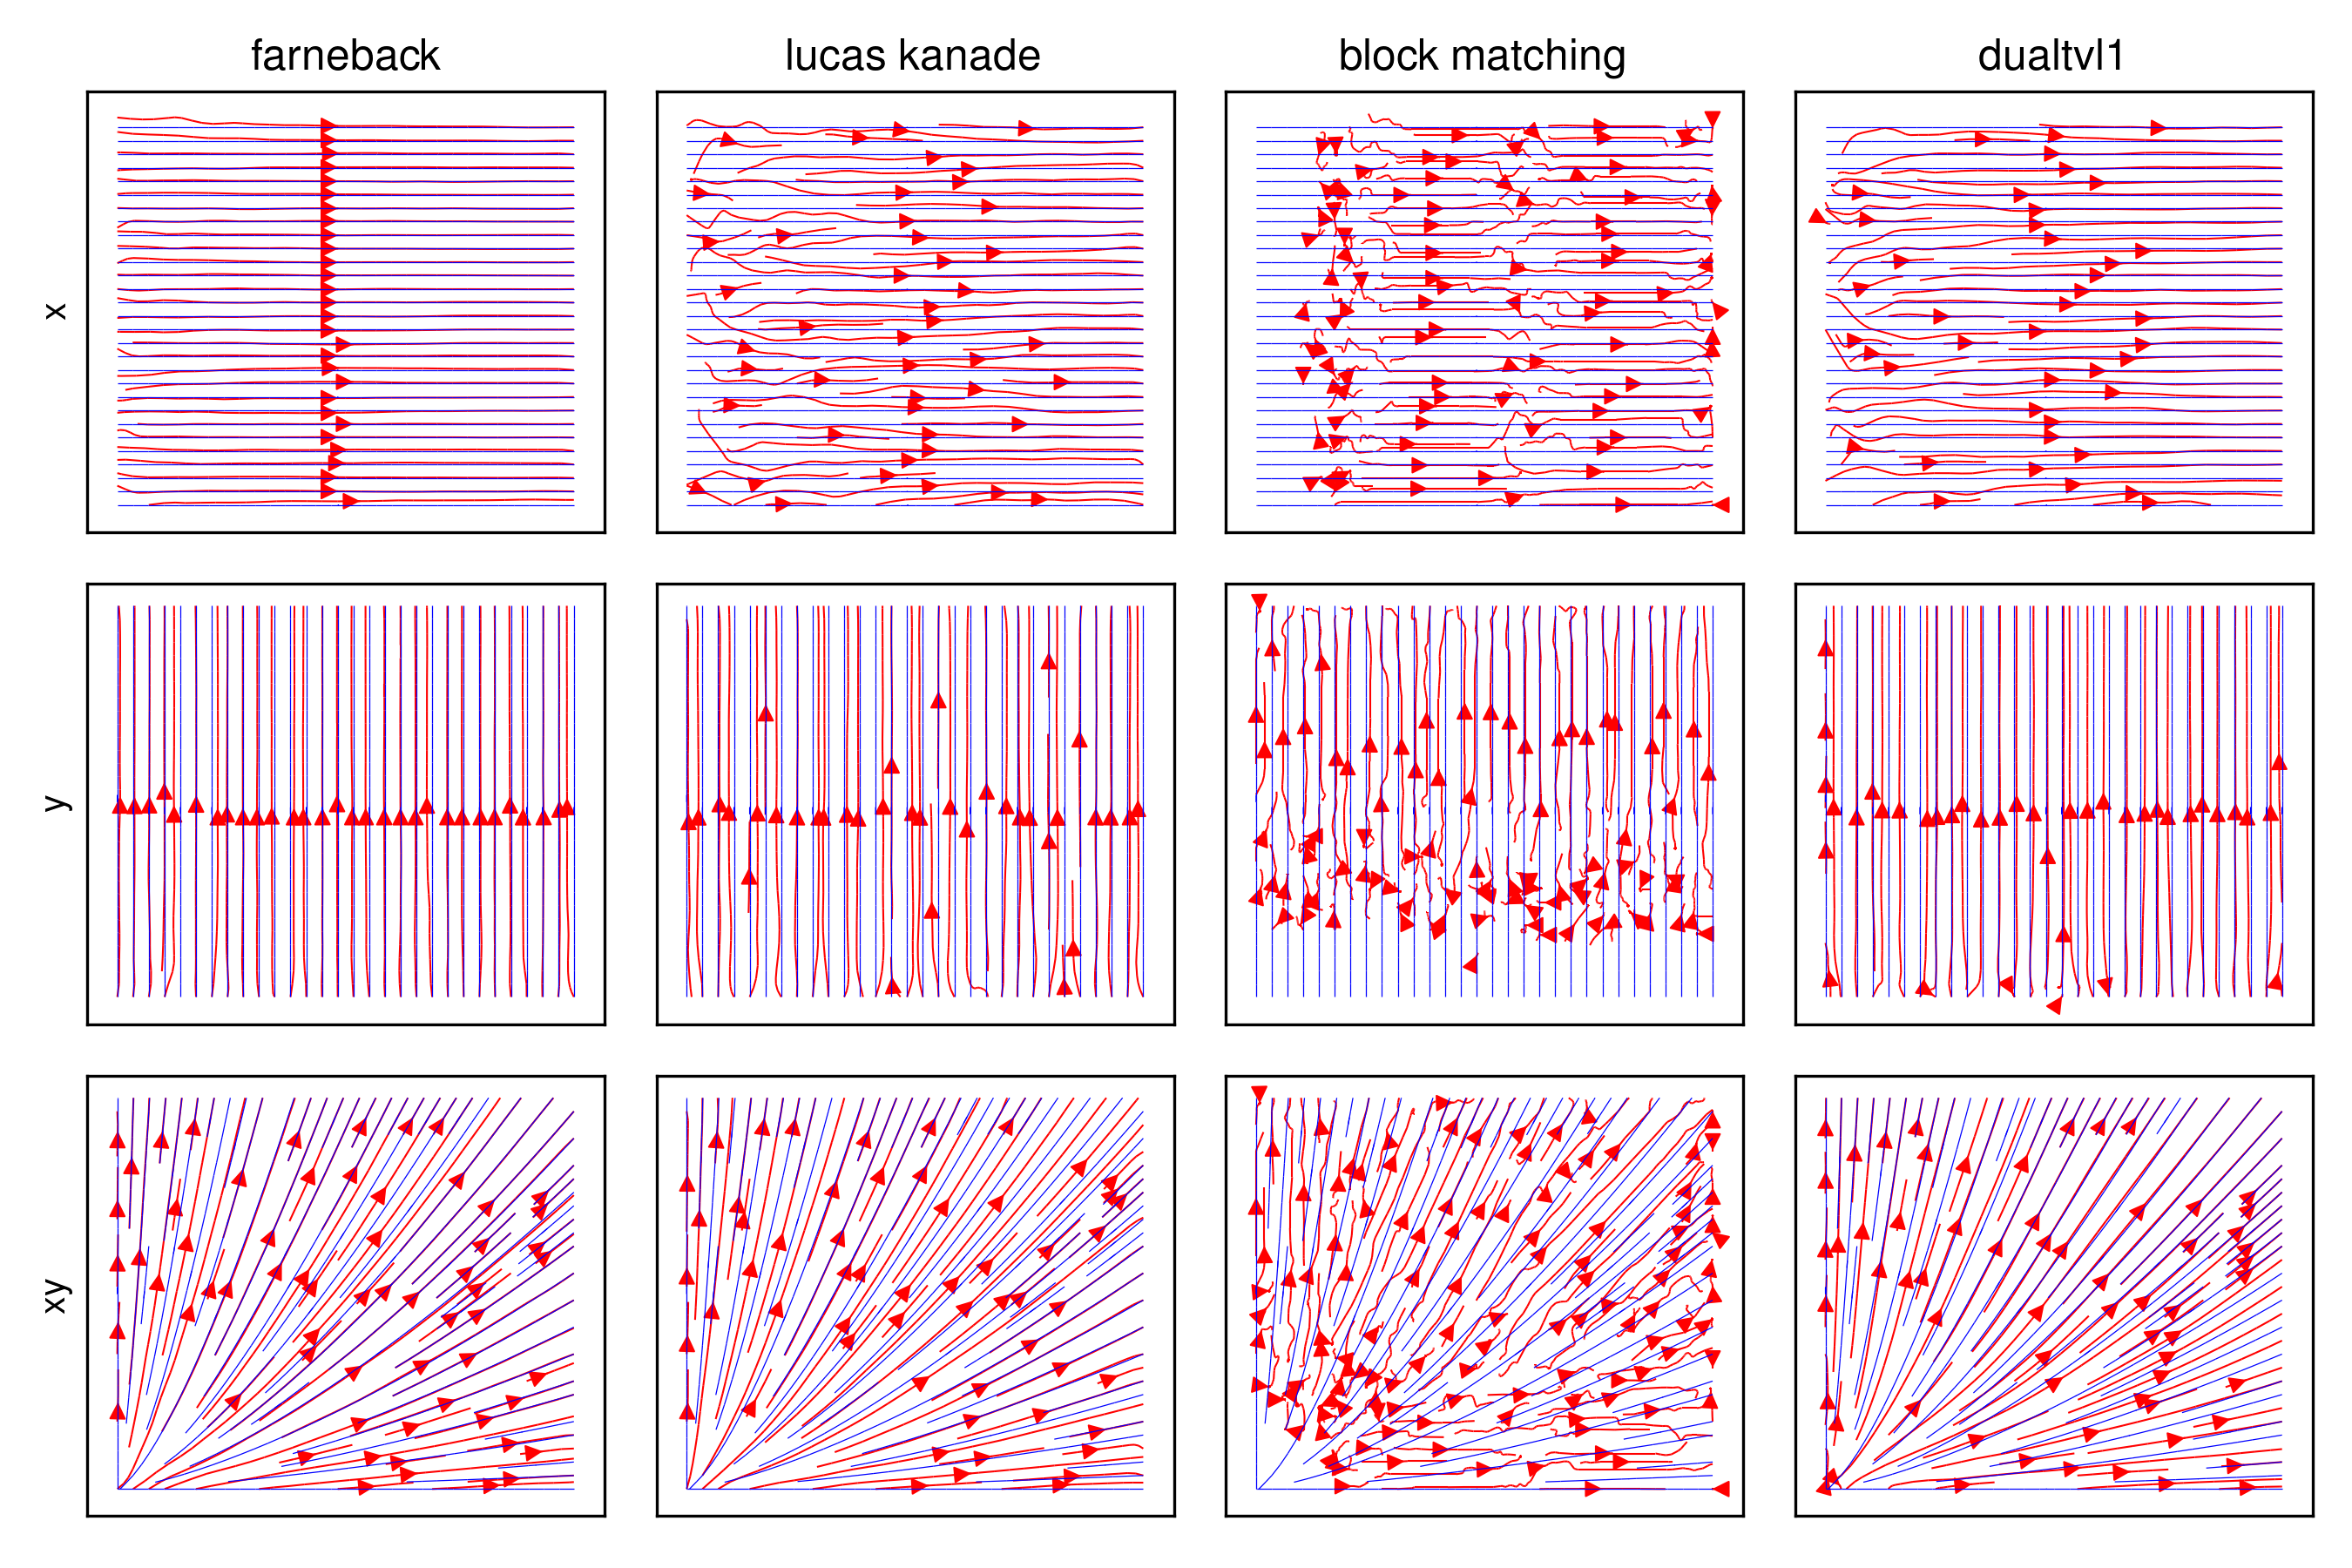
\includegraphics[width=\textwidth]{figures/known_displacement_algs.png}
\end{minipage}\hfill
\begin{minipage}[t]{5.5in}
\vspace{5mm}
\bigskip
\textbf{$\triangleleft$ Figure:}
\begin{enumerate}
    \item We tested four  optical flow algorithms (Farneback, Lucas-Kanade, Block Matching[1] and Duial TV-L1) on a three different toy problems with known displacement.
    \item The streamlines show the true displacement, while the arrows show the estimated displacement.
    \item Among the algorithms tested, the Farneback method[2] performed best.
\end{enumerate}

\end{minipage}
\end{minipage}};

\node[anchor=east, rounded corners=3mm, fill=simula]
(optflow title)
at ($ (optflow.north east)!3cm!(optflow.north west) $)
{\ffmfamily Optical flow algorithm};

%%%% Feature calculation %%%%
\node[draw=simula, line width=1mm, anchor=north west,
      rounded corners=4mm, inner sep=1cm,
      fill=simula!10!white, minimum height=10cm]
(feature)
at ($(optflow.north east)+(1cm,0)$)
{\begin{minipage}{14.5in}
\footnotesize

From the optical flow solution we can compute the displacement and velocity traces by averaging over the pixels.

\begin{minipage}[t]{0.48\textwidth}
\vspace{0pt}
\begin{center}
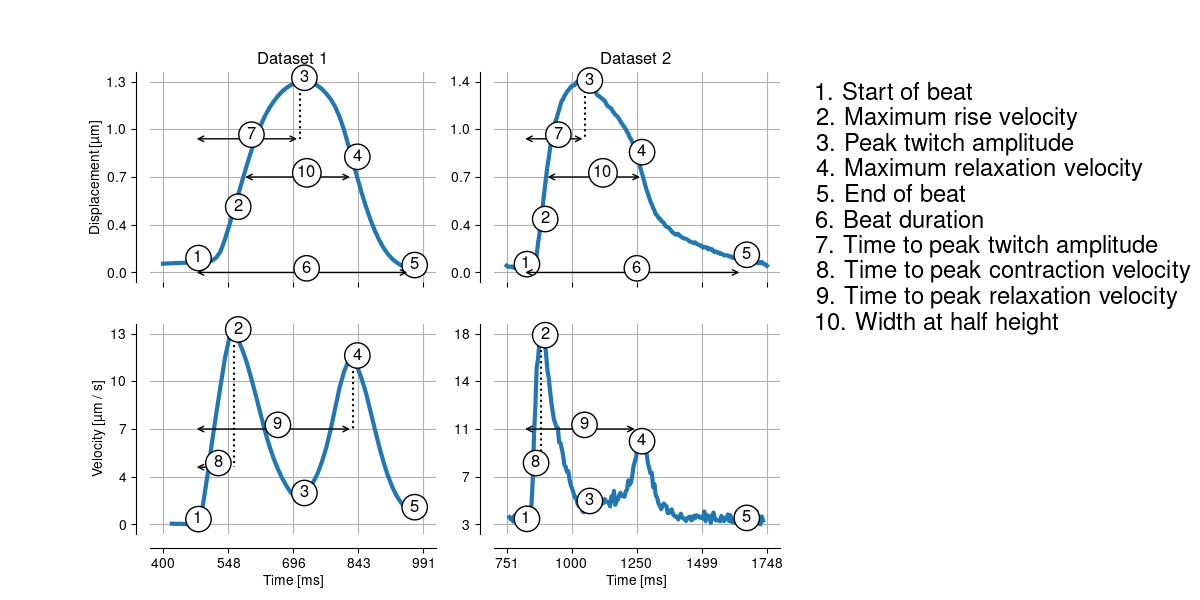
\includegraphics[width=\textwidth]{figures/disp_velocity_first_beat.png}    
\end{center}
\textbf{$\triangle$ Figure:}
We computed  features on the resulting displacement and velocity traces. Here we show example values for two different analyzed samples.
\end{minipage}\hfill
\begin{minipage}[t]{0.5\textwidth}
\vspace{5mm}
\bigskip
\begin{tabular}{lrr}
\toprule
Name & Dataset 1 & Dataset 2 \\
\midrule
Maximum rise velocity [$\mu$m/s] & 13.4 & 18.0 \\
Peak twitch amplitude [$\mu$m]  & 1.3 & 1.4 \\
Maximum relaxation velocity [$\mu$m/s] & 11.6 & 9.2 \\
Beat duration [ms]  & 494.1 & 852.0 \\
Time to peak twitch amplitude [ms] & 320.2 & 276.0 \\
Time to peak contraction velocity [ms] & 102.9 & 16.3 \\
Time to peak relaxation velocity [ms] & 373.1 & 382.3 \\
Width at half height [ms] & 258.2 & 371.8 \\
Start of beat [ms] & 437.5 & 859.7 \\
End of beat [ms] & 931.6 & 1711.8 \\
\bottomrule
\end{tabular}
\end{minipage}
\end{minipage}};

\node[anchor=west, rounded corners=3mm, fill=simula]
(feature title)
at ($ (feature.north west)!3cm!(feature.north east) $)
{\ffmfamily Feature calculations};

%%%% Sensitivity analysis %%%%
\node[draw=simula, line width=1mm, anchor=north west,
      rounded corners=4mm, inner sep=1cm,
      fill=simula!10!white, minimum height=17.5in]
(sensitivity)
at ($(optflow.south west)+(0,-2cm)$)
{\begin{minipage}{12in}
\footnotesize
\vfill
\vspace{0.3cm}
The computations needed to perform motion estimation are both computationally expensive and prone to errors. Here we show result of filtering the motion vectors, timings for the different operations as well as some local differences in the displacement and velocity.

\begin{minipage}[t]{0.4\textwidth}
\vskip0pt
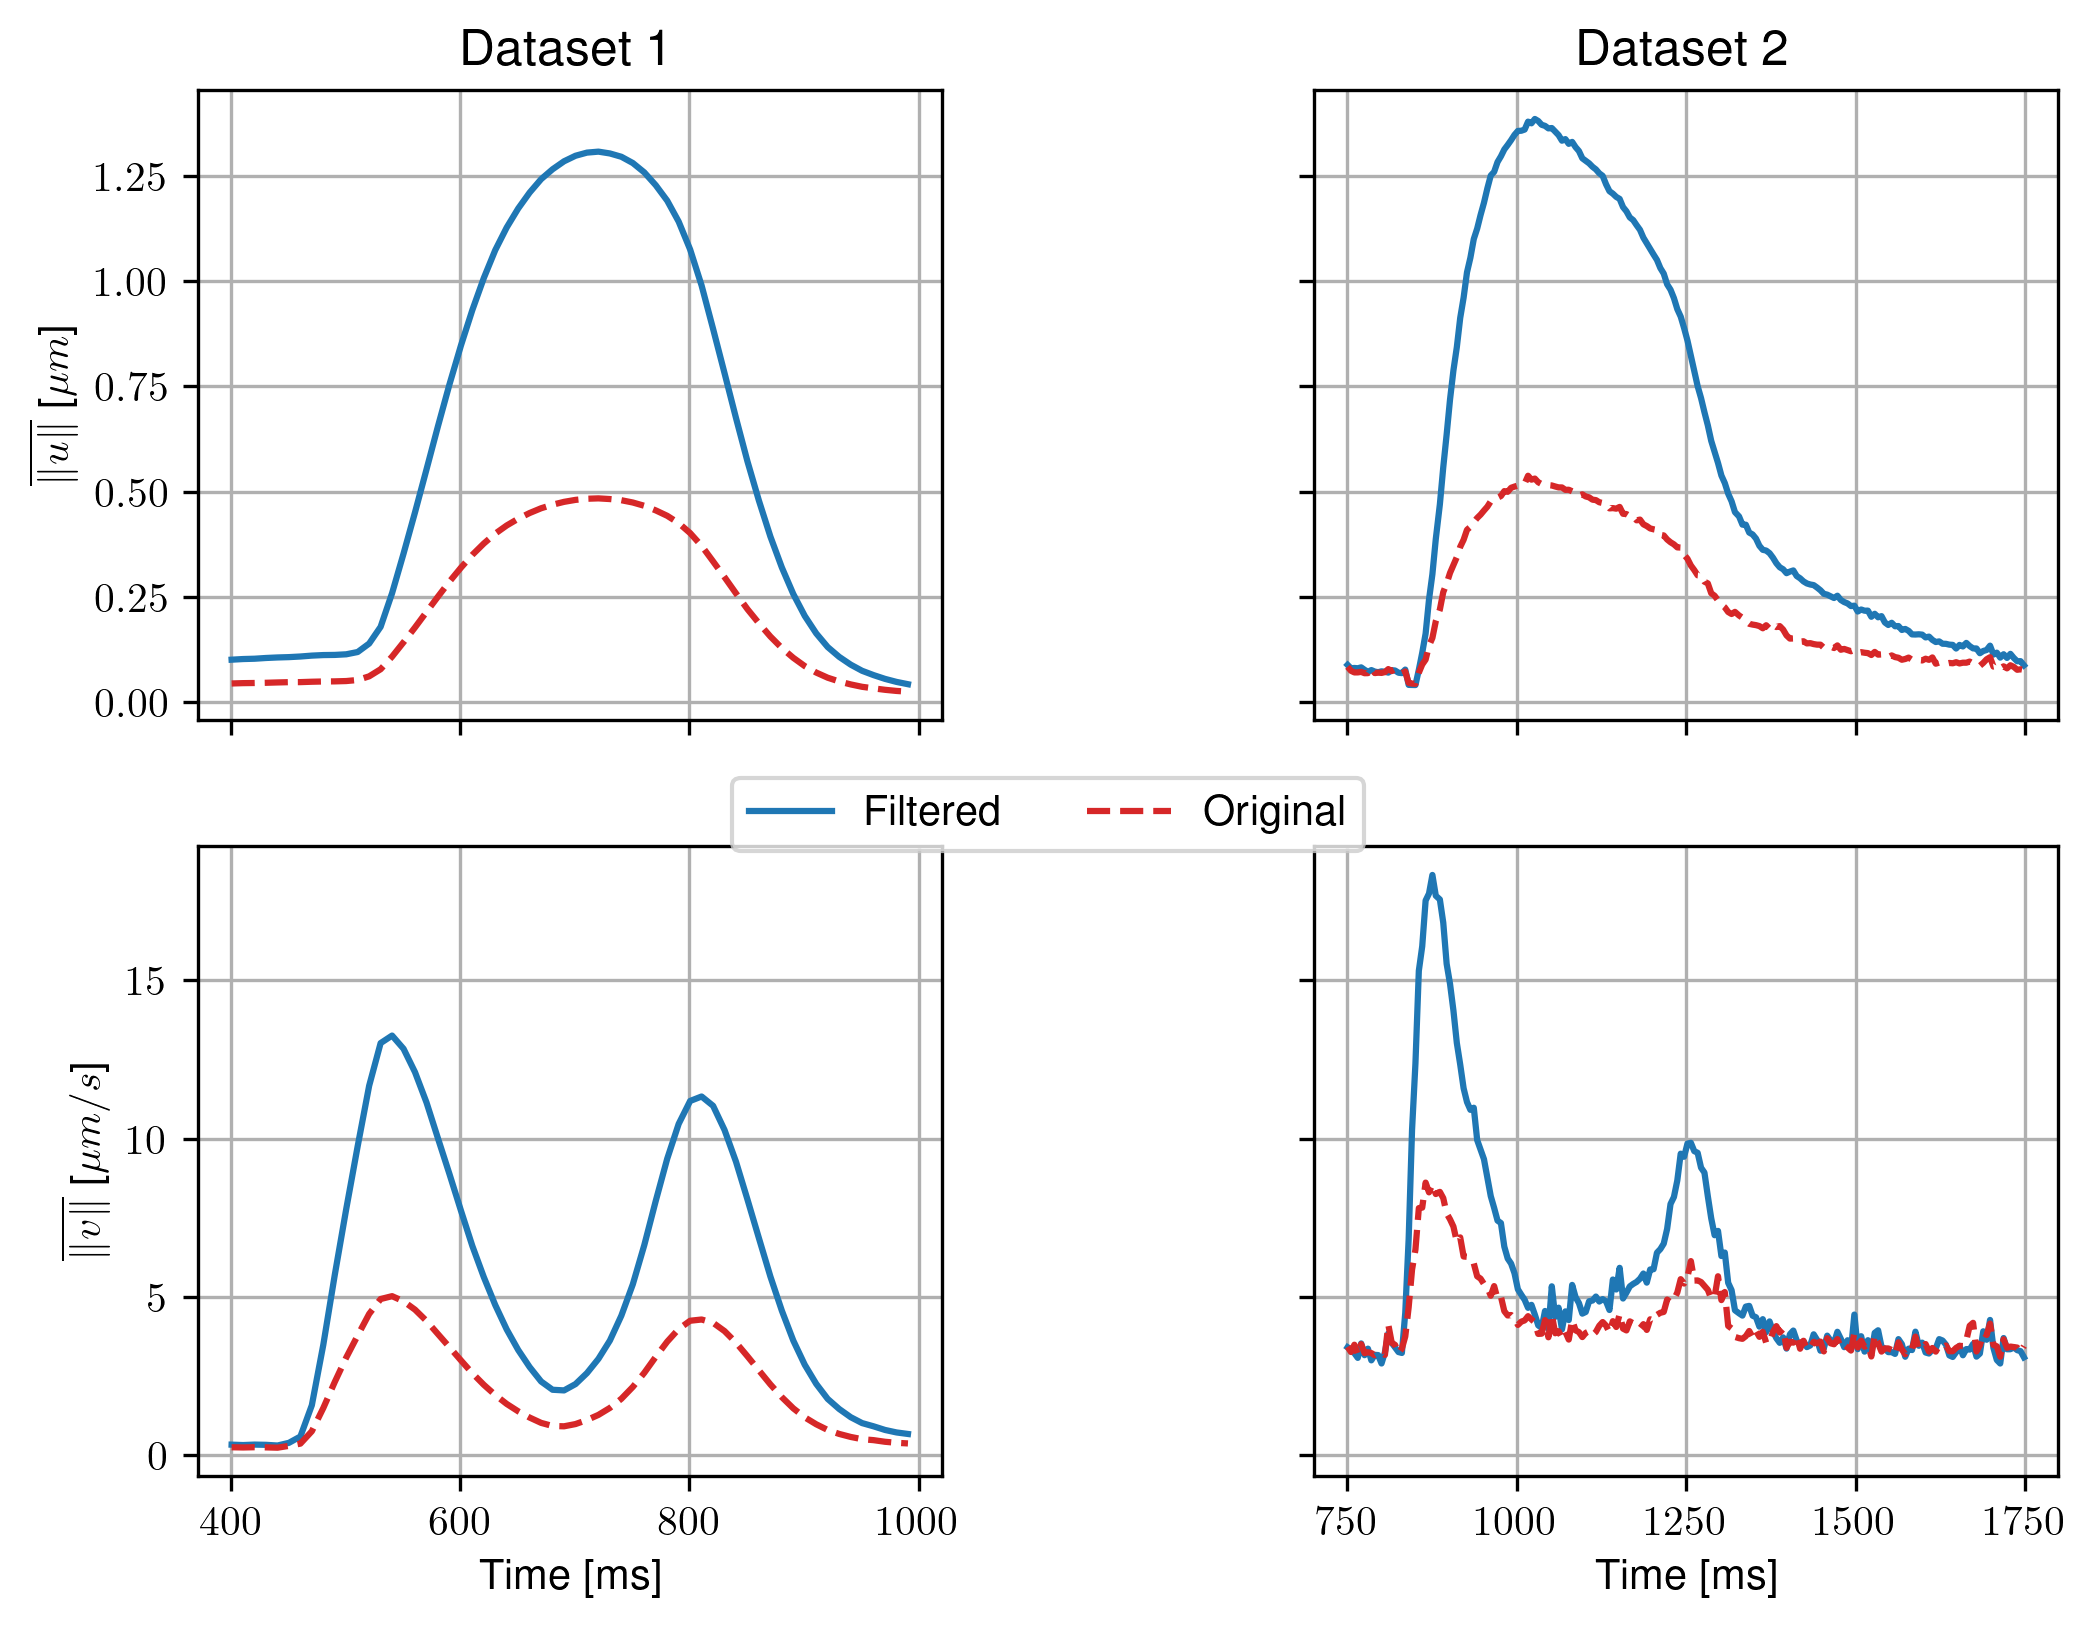
\includegraphics[width=\textwidth]{figures/filtered_traces_simple.png}
\end{minipage}\hfill
\begin{minipage}[t]{0.58\textwidth}
\vskip0pt
\textbf{$\triangleleft$ Figure:}
We apply a filtering to the displacement and velocity in order to remove pixels with a low maximum displacement. Pixels with small maximum displacement are likely to be either pixels that does not contain cardiomyocytes, or they contain cardiomyocytes that are not contributing to the overall displacement. In these cases the signal from these pixels could potentially corrupt the resulting motion vector directions [1]. This is not a big problem for displacement vectors, since all displacement vectors are computed relative to one reference frame. However, for the velocity vectors this can result in very rapid changes in the directions of the vectors.
\end{minipage}
\vfill
\vspace{0.3cm}
\begin{minipage}[t]{0.96\textwidth}
\vskip0pt
\textbf{$\triangle$ Figure:} When applying the filtering, pixels with low displacement magnitude are excluded from the mean computation. The means that averages are now computed over the pixels with higher displacement values and it will thus result in a higher mean displacement. It is also clear that by applying filtering we exclude pixels that only contribute to noise in the signals, and thus the noise level in the filtered signal is reduced.
\end{minipage}

\vspace{1cm}
\begin{minipage}[t]{0.35\textwidth}
\vskip0pt
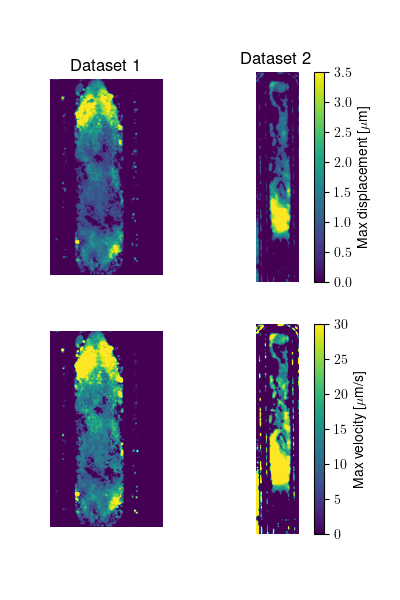
\includegraphics[width=\textwidth]{figures/max_disp_vel_norm.png}
\vskip0pt
\textbf{$\triangle$ Figure:} 
We computed the maximum velocity and displacement over all time steps for the two datasets, and found large regional variations.
\end{minipage}\hfill
\begin{minipage}[t]{0.63\textwidth}
\vskip0pt
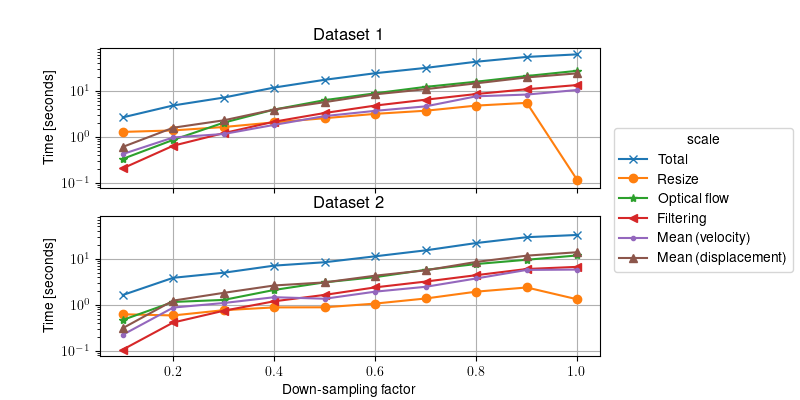
\includegraphics[width=\textwidth]{figures/timings_scale.png}
\vskip0pt
\textbf{$\triangle$ Figure:} Timings for the different operations during motion analysis. \emph{Resize} is the time spent down-sampling the data from original size of a lower resolution. \emph{Optical flow} is the time spent running the Farneback method, \emph{Filtering} is the time spent computing the mask and applying the filtering to both displacement and velocity. Finally \emph{mean (X)} is the time spent of computing the norm and mean of all the arrays for X (X being velocity and displacement). The blue line also show the total time spent for each resolution. 
\end{minipage}
\end{minipage}};

\node[anchor=west, rounded corners=3mm, fill=simula]
(sensitivity title)
at ($ (sensitivity.north west)!3cm!(sensitivity.north east) $)
{\ffmfamily Sensitivity analysis, local variation and timings};

%%%% Sentitity analysis

\node[draw=simula, line width=1mm, anchor=north west,
      rounded corners=4mm, inner sep=1cm,
      fill=simula!10!white, minimum height=20in]
(drug)
at ($(feature.south west)+(0,-2cm)$)
{\begin{minipage}{14.5in}
\footnotesize

We tested the library on two different drugs that are known to affect the mechanics of cardiac cells, specifically using bay K 8644 and omecamtiv mercarbil.


\begin{minipage}[t]{\textwidth}
\vskip0pt
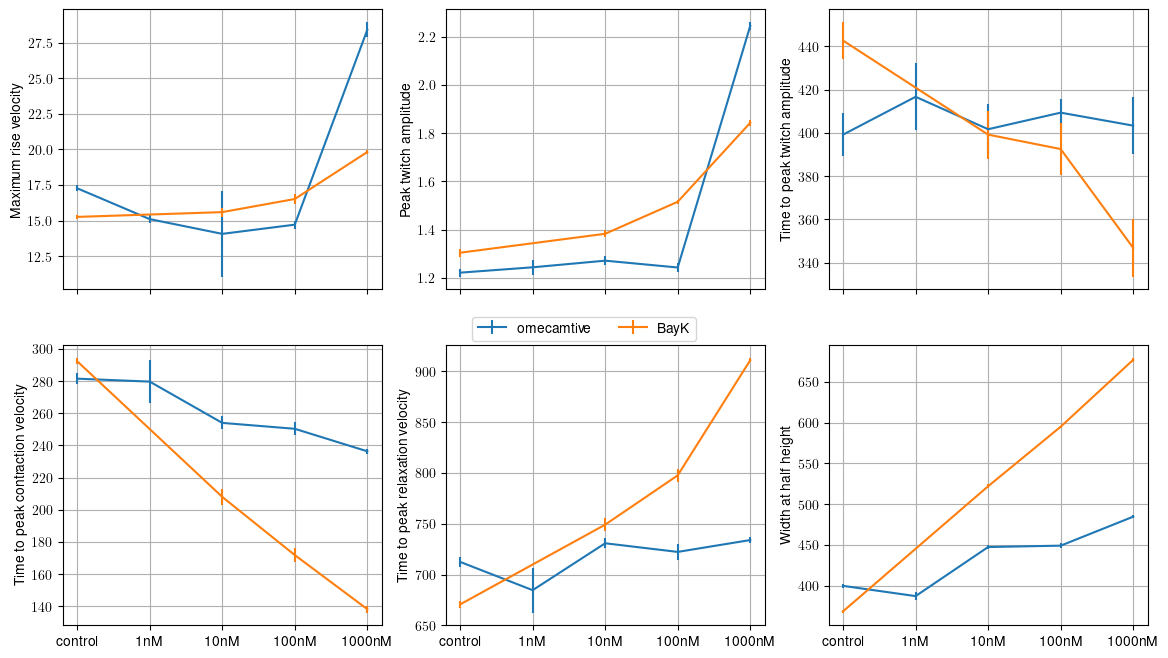
\includegraphics[width=\textwidth]{figures/features.png}
\textbf{$\triangle$ Figure:} 
Different features for increasing dose of  BayK and Omecamtiv.
\end{minipage}
\vfill
\vspace{1cm}
Both voltage, calcium and motion data where aligned and plotted for each dose of the drugs.

{\begin{minipage}[t]{\textwidth}
\footnotesize
\begin{minipage}[t]{0.49\textwidth}
\vskip0pt
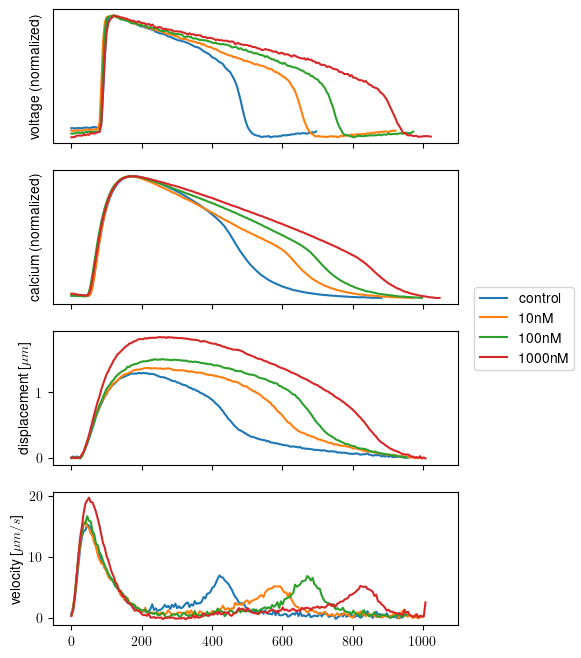
\includegraphics[width=\textwidth]{figures/BayK.png}
\textbf{$\triangle$ Figure:}
Voltage, calcium, displacement and velocity for different doses of BayK
\end{minipage}
\hfill
\begin{minipage}[t]{0.49\textwidth}
\vskip0pt
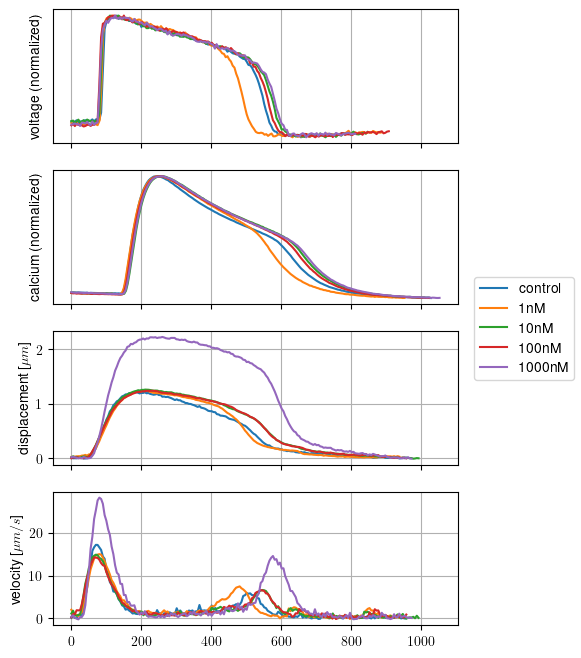
\includegraphics[width=\textwidth]{figures/omecamtiv.png}
\textbf{$\triangle$ Figure:}
Voltage, calcium, displacement and velocity for different doses of Omecamtiv
\end{minipage}
\end{minipage}};

\end{minipage}};

\node[anchor=east, rounded corners=3mm, fill=simula]
(drug title)
at ($ (drug.north east)!3cm!(drug.north west) $)
{\ffmfamily Drug escalation study};

We tested the library on two different drugs that are known to affect the mechanics of cardiac cells, i.e BayK and Omecamtiv.


%%%% References %%%%

\node[draw=none, anchor=north west]
(references)
at ($(drug.south west)+(0,-1cm)$)
{\begin{minipage}{14.5in}


\begin{minipage}[t]{\textwidth}

{\bfseries\ffmfamily\Large\underline{References}};
\vfill
\vspace{1cm}
\footnotesize
[1] Huebsch, N et al. Metabolically-Driven Maturation of hiPSC-Cell Derived Cardiac Chip. Biorxiv (preprint). 2020. https://doi.org/10.1101/485169.

\medskip
[2] Farnebäck, Gunnar. "Two-frame motion estimation based on polynomial expansion." Scandinavian conference on Image analysis. Springer, Berlin, Heidelberg, 2003.
\end{minipage}

\end{minipage}};



%%%% footer %%%%
\begingroup
\pgfmathsetseed{31417}
\fill[simula,
      drop shadow={shadow yshift=1ex, shadow xshift=-1ex}]
decorate[decoration={random steps, segment length=1cm, amplitude=4mm}]
{ ($(current bounding box.south west)+(-1cm,4cm)$) --
  ($(current bounding box.south east)+(1cm,4cm)$) }
-- (current bounding box.south east) --
   (current bounding box.south west) -- cycle;
\node[anchor=west]
at ( $(current bounding box.south west)+(1cm,2cm)$ )
{
\includegraphics[height=2cm]{simula_logo_main_black}};
\endgroup

\end{tikzpicture}

\end{document}
